% 第3章第2节：Poisson方程与弱解（从边值问题到弱形式；存在唯一与能量估计；其他边界条件与非唯一性）。

\section{Poisson方程与弱解}
\label{sec:pde-poisson}

本节研究不随时间变化的场。稳态温度、静电势、受载薄膜的位移都满足\term{Poisson方程}（Poisson equation）$-\Delta u=f$，其中$f$是源项。我们借这个方程完整走一遍三步：先把它改写成用测试函数检验的弱形式，再证明弱解存在唯一并用数据控制解，最后看边界条件改变时这些结论怎样随之改变。后面的热方程、波动方程和有限元方法都会沿用这里的弱形式与能量估计。

\subsection{从边值问题到弱形式}
\label{sec:pde-weak-form}

\paragraph{一维边值问题与Green函数}
先看能直接求解的情形：在$(0,1)$上求$u$，使
\begin{equation}
  -u''=f\quad\text{于}(0,1),\qquad u(0)=u(1)=0 .
  \label{eq:pde-poisson-1d}
\end{equation}
它描述两端固定、受分布载荷$f$的弦的平衡位移，也描述两端保持零度、有热源$f$的棒的稳态温度。对连续的$f$，积分两次并用边界条件定常数，可以把解写成
\begin{equation}
  u(x)=\int_0^1G(x,y)f(y)\,\mathrm dy,\qquad
  G(x,y)=\begin{cases}x(1-y),&0\leq x\leq y,\\ y(1-x),&y\leq x\leq1 .\end{cases}
  \label{eq:pde-green-1d}
\end{equation}
直接验证：$u(x)=(1-x)\int_0^xyf(y)\,\mathrm dy+x\int_x^1(1-y)f(y)\,\mathrm dy$，求导时两处边界项$\pm x(1-x)f(x)$互相抵消，得$u'(x)=-\int_0^xyf(y)\,\mathrm dy+\int_x^1(1-y)f(y)\,\mathrm dy$，再求导得$u''(x)=-xf(x)-(1-x)f(x)=-f(x)$；又$u(0)=u(1)=0$。函数$G$称为这个边值问题的\term{Green函数}（Green's function）。

$G(\cdot,y)$本身有清楚的含义：它是在$y$处放一个单位点热源时的稳态温度，形状是在$y$处取得最大值$y(1-y)$的“帐篷”。式~\eqref{eq:pde-green-1d}说，分布热源产生的温度是各点点源效应的叠加。图~\ref{fig:pde-poisson-energy}(a)画出三种总热量都为$1$的源：均匀源$f=1$给出$u=x(1-x)/2$，最高温$1/8$；只加热中段的$f=2\cdot\mathbf 1_{[1/4,3/4]}$给出最高温$3/16$；集中在中点的点源给出帐篷$G(\cdot,1/2)$，最高温$1/4$。热量越集中，中点越热。

式~\eqref{eq:pde-green-1d}的右端只需要$f$可积就有意义。对$f=2\cdot\mathbf 1_{[1/4,3/4]}$，上面$u'$的表达式仍然成立且连续，$u''=-f$在除$x=1/4,3/4$两点外成立。上一节已经说明这样的$u$不是经典解；点源的帐篷在$x=1/2$处连一阶导数都没有。这些物理上合理的“解”都需要一种新的检验方式。

\paragraph{用测试函数检验方程}
设$u$是式~\eqref{eq:pde-poisson-1d}的经典解，$\varphi\in C_c^\infty(0,1)$是测试函数。两边乘以$\varphi$再积分，用分部积分把一个导数从$u$移到$\varphi$上：
\[
  \int_0^1f\varphi\,\mathrm dx=-\int_0^1u''\varphi\,\mathrm dx
  =\int_0^1u'\varphi'\,\mathrm dx-\bigl[u'\varphi\bigr]_0^1
  =\int_0^1u'\varphi'\,\mathrm dx .
\]
边界项消失，因为$\varphi$在两端附近为零。右端只用到$u$的一阶导数，而$u$的二阶导数已经转移给了光滑的$\varphi$。

不妨把$\varphi$想成一个探针：把它放在某处，读出方程两边在这一小段上的加权平均。经典解要求方程在每一点成立；弱的检验只要求每一个探针读到的两个平均值相等。探针足够多时，这两种要求并不矛盾，因为与所有测试函数积分都相同的两个局部可积函数几乎处处相等。图~\ref{fig:pde-weak-form-test}用一个带尖点的函数说明这种转移：$u=\tfrac12-|x-\tfrac12|$在$x=1/2$处没有经典导数，弱导数$u'$是一个跳跃的阶梯；$u'\varphi$与$-u\varphi'$是两个完全不同的函数，积分却相等，都约为$-0.040$。

\begin{figure}[!htb]
  \centering
  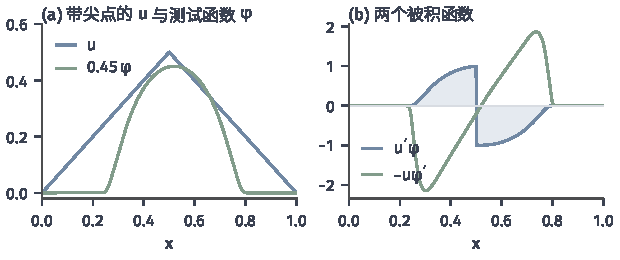
\includegraphics[width=105mm]{figures/03-optimization-evolution-and-signals/02-processes-and-trajectory-evolution/matplotlib/pde-weak-form-test/figure.pdf}
  \caption{把导数转移到测试函数上。(a)~$u=\tfrac12-|x-\tfrac12|$在$x=1/2$处有尖点；测试函数$\varphi$光滑，只在$(0.22,0.82)$内非零，图中缩小为$0.45$倍。(b)~两个被积函数：$u'\varphi$在尖点处跳跃（阴影），$-u\varphi'$连续；二者的积分在数值上都约为$-0.040$（梯形求积，$40001$个点）。}
  \label{fig:pde-weak-form-test}
\end{figure}

在$d$维有界区域上做同样的事，需要多元的分部积分。对向量场$v\nabla u$用散度定理，并利用$\nabla\cdot(v\nabla u)=\nabla v\cdot\nabla u+v\Delta u$，得到\term{Green第一恒等式}（Green's first identity）
\begin{equation}
  \int_\Omega(-\Delta u)\,v\,\mathrm d\bm x
  =\int_\Omega\nabla u\cdot\nabla v\,\mathrm d\bm x-\int_{\partial\Omega}(\partial_{\bm n}u)\,v\,\mathrm dS,
  \label{eq:pde-green-identity}
\end{equation}
它对有界Lipschitz区域、$u\in C^2(\overline\Omega)$与$v\in C^1(\overline\Omega)$成立。光滑边界上的散度定理（Gauss公式）及Laplace算子可参考\BookChapterRef{chap:multivariate-integration}{卷一“多元函数积分”章}；推广到Lipschitz边界需要几乎处处存在的外法向，这里不加证明地使用。若$v$在边界上为零，边界项消失，左边的二阶导数就变成了右边两个一阶导数的配对。

\paragraph{弱形式的定义}
式~\eqref{eq:pde-green-identity}提示：零Dirichlet边界的Poisson问题应当在$H_0^1(\Omega)$中寻找解，并用$H_0^1(\Omega)$中的函数检验。源项则只需要作为$H_0^1(\Omega)$上的连续线性泛函出现。由Poincaré不等式，$\|\nabla v\|$在$H_0^1(\Omega)$上与$H^1$范数等价，我们取它为$H_0^1(\Omega)$的范数，并把$H_0^1(\Omega)$上全体有界线性泛函组成的空间记为$H^{-1}(\Omega)$，范数为
\[
  \|\ell\|_{H^{-1}}=\sup_{v\in H_0^1(\Omega),\,v\neq0}\frac{|\ell(v)|}{\|\nabla v\|} .
\]

\begin{definition}[零Dirichlet边界Poisson问题的弱解]
\label{def:pde-weak-dirichlet}
设$\Omega\subset\mathbb R^d$为有界开集，$\ell\in H^{-1}(\Omega)$。若$u\in H_0^1(\Omega)$满足
\begin{equation}
  a(u,v):=\int_\Omega\nabla u\cdot\nabla v\,\mathrm d\bm x=\ell(v)\qquad\text{对所有}v\in H_0^1(\Omega),
  \label{eq:pde-weak-dirichlet}
\end{equation}
称$u$为$-\Delta u=\ell$在零Dirichlet边界条件下的弱解。$\ell(v)=\langle f,v\rangle$、$f\in L^2(\Omega)$时，也说$u$是$-\Delta u=f$的弱解。式~\eqref{eq:pde-weak-dirichlet}称为问题的\term{弱形式}（weak formulation）。
\end{definition}

定义里有三个选择，各有理由。第一，边界条件写进了解空间：$u\in H_0^1(\Omega)$在Lipschitz区域上就是迹为零。第二，检验函数取整个$H_0^1(\Omega)$而不只是$C_c^\infty(\Omega)$：两边对$v$都在$H^1$范数下连续，而$C_c^\infty(\Omega)$按定义在$H_0^1(\Omega)$中稠密，所以对测试函数成立等价于对全体$H_0^1$函数成立；扩大检验范围是为了下面能取$v=u$。第三，$f\in L^2(\Omega)$确实给出$H^{-1}$中的元素：由Cauchy--Schwarz与Poincaré不等式，
\[
  |\langle f,v\rangle|\leq\|f\|\,\|v\|\leq C_P\|f\|\,\|\nabla v\|,\qquad\text{故}\quad\|f\|_{H^{-1}}\leq C_P\|f\| .
\]

\begin{example}[一维点源是$H^{-1}$中的元素]
\label{ex:pde-point-source}
在$(0,1)$上固定$y$，令$\ell(v)=v(y)$，即点源只读取$v$在$y$处的值。$H_0^1(0,1)$的函数有连续代表且$v(0)=0$，所以$|v(y)|=|\int_0^yv'|\leq\sqrt y\,\|v'\|$，$\ell$有界，$\|\ell\|_{H^{-1}}\leq\sqrt y$。Green函数$u=G(\cdot,y)$就是对应的弱解：$G(\cdot,y)$在$(0,y)$上斜率为$1-y$，在$(y,1)$上斜率为$-y$，于是对任意$v\in H_0^1(0,1)$，
\[
  \int_0^1G_x(x,y)v'(x)\,\mathrm dx=(1-y)\bigl(v(y)-v(0)\bigr)-y\bigl(v(1)-v(y)\bigr)=v(y) .
\]
在$d\geq2$时情形不同：$H^1$函数可以在一点附近无界，读取点值不是$H_0^1$上的有界泛函，点源不属于$H^{-1}(\Omega)$，需要另外的解释。
\end{example}

\paragraph{经典解与弱解的关系}
弱解是经典解的推广，而不是另一个问题。下面的结论说明，在光滑的情形两种解释给出同一个对象。

\begin{theorem}[经典解与弱解]
\label{thm:pde-classical-weak}
设$\Omega$为有界Lipschitz区域，$f\in C(\overline\Omega)$。
\begin{enumerate}
  \item 若$u\in C^2(\overline\Omega)$在$\Omega$内满足$-\Delta u=f$，在$\partial\Omega$上$u=0$，则$u$是定义~\ref{def:pde-weak-dirichlet}意义下的弱解。
  \item 若弱解$u$还属于$C^2(\overline\Omega)$，则它在$\Omega$内处处满足$-\Delta u=f$，在$\partial\Omega$上处处为零。
\end{enumerate}
\end{theorem}

\begin{proof}
(1)~$u\in C^1(\overline\Omega)$，所以$u\in H^1(\Omega)$，其迹等于边界限制，为零；由零迹刻画，$u\in H_0^1(\Omega)$。对$v\in C_c^\infty(\Omega)$，式~\eqref{eq:pde-green-identity}的边界项为零，得$a(u,v)=\langle f,v\rangle$。两边对$v$在$H^1$范数下连续，由稠密性推广到全部$v\in H_0^1(\Omega)$。

(2)~对$\varphi\in C_c^\infty(\Omega)$，由式~\eqref{eq:pde-green-identity}与弱形式，$\int_\Omega(-\Delta u-f)\varphi\,\mathrm d\bm x=a(u,\varphi)-\langle f,\varphi\rangle=0$。连续函数$-\Delta u-f$与所有测试函数的积分为零，几乎处处为零，由连续性处处为零。又$u\in C^1(\overline\Omega)$时迹就是边界限制，而$u\in H_0^1(\Omega)$的迹为零，所以$u$在$\partial\Omega$上为零。
\end{proof}

\paragraph{与能量极小的对应}
弱形式还有一个能量的读法。定义
\begin{equation}
  J(v)=\frac12\int_\Omega|\nabla v|^2\,\mathrm d\bm x-\ell(v),\qquad v\in H_0^1(\Omega).
  \label{eq:pde-dirichlet-energy}
\end{equation}
对弦来说，第一项是拉伸储存的弹性能，第二项是载荷所做的功。展开平方，对任意$u,w\in H_0^1(\Omega)$，
\begin{equation}
  J(u+w)=J(u)+\bigl[a(u,w)-\ell(w)\bigr]+\frac12\|\nabla w\|^2 .
  \label{eq:pde-energy-expansion}
\end{equation}
若$u$是弱解，方括号对所有$w$为零，于是$J(u+w)=J(u)+\tfrac12\|\nabla w\|^2$；由Poincaré不等式，$\|\nabla w\|=0$迫使$w=0$，所以$u$是$J$的唯一最小点。反过来，若$u$最小化$J$，则一元二次函数$s\mapsto J(u+sw)$在$s=0$处取最小值，它在$s=0$处的导数正是方括号，必须为零，这就是弱形式。所以对这个对称问题，“弱解”与“能量最小点”是同一件事；弱形式是能量的一阶条件，在函数层面写出来就是$J$的\term{Euler--Lagrange方程}（Euler--Lagrange equation）。

图~\ref{fig:pde-poisson-energy}(b)沿两个方向画出了$f=1$时的$J(u+sw)$：每条都是开口向上的抛物线，最低点都在$s=0$，最低值都是$J(u)=-1/24$。曲率是$\|\nabla w\|^2$，$w=\sin(3\pi x)$的曲率是$w=\sin(\pi x)$的$9$倍，振荡越快的扰动付出的弹性能越大。

\begin{figure}[!htb]
  \centering
  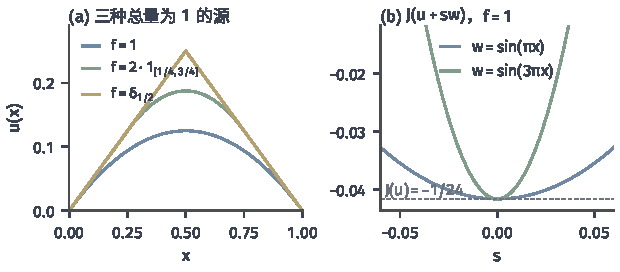
\includegraphics[width=105mm]{figures/03-optimization-evolution-and-signals/02-processes-and-trajectory-evolution/matplotlib/pde-poisson-energy/figure.pdf}
  \caption{一维Poisson问题~\eqref{eq:pde-poisson-1d}。(a)~三种总量为$1$的源对应的解：均匀源、中段加热与中点的点源，由Green函数~\eqref{eq:pde-green-1d}计算，最高值分别为$1/8$、$3/16$、$1/4$。(b)~$f=1$时能量~\eqref{eq:pde-dirichlet-energy}沿两个方向的截面$J(u+sw)=-\tfrac1{24}+\tfrac{s^2}{2}\|w'\|^2$，最小点都在$s=0$。}
  \label{fig:pde-poisson-energy}
\end{figure}

第~\ref{chap:optimization}章在有限维中证明过：可微凸函数的驻点就是全局最小点，强凸时最小点唯一。$J$是Hilbert空间上的二次凸函数，上面的展开是同一个结构的直接计算。可是有限维中证明最小点\emph{存在}所用的论证，即下水平集有界闭从而紧，在$H_0^1(\Omega)$中失效：无限维空间的有界闭集一般不紧。写出Euler--Lagrange方程只说明“如果有最小点，它满足什么”，并没有证明最小点或弱解存在，也没有说明数据怎样控制解。下一小节回答这两个问题。

\subsection{存在唯一与能量估计}
\label{sec:pde-lax-milgram}

\paragraph{双线性型与强制性}
把弱形式~\eqref{eq:pde-weak-dirichlet}抽象出来：$V$是实Hilbert空间，范数$\|\cdot\|_V$；$a:V\times V\to\mathbb R$对每个变量都是线性的，称为\term{双线性型}（bilinear form）；$\ell\in V'$是有界线性泛函。我们要求$u\in V$，使$a(u,v)=\ell(v)$对所有$v\in V$成立。两个条件将起关键作用：
\begin{equation}
  |a(u,v)|\leq M\|u\|_V\|v\|_V,\qquad a(v,v)\geq\alpha\|v\|_V^2,\qquad u,v\in V,
  \label{eq:pde-bounded-coercive}
\end{equation}
其中$M,\alpha>0$为常数。前者是有界性，后者称为$a$的\term{强制性}（coercivity）。在$V=\mathbb R^n$中，$a(u,v)=\bm v^{\top}\bm K\bm u$，强制性就是$\bm v^{\top}\bm K\bm v\geq\alpha\|\bm v\|_2^2$：沿任何方向推动，$a$都给出与推动量平方成比例的正回应。这样的矩阵没有非零零向量，因而可逆。下面要在无限维中得到同样的结论。

\paragraph{对称情形：Riesz表示}
若$a$还是对称的，$a(u,v)=a(v,u)$，则$(u,v)_a:=a(u,v)$是$V$上的内积。式~\eqref{eq:pde-bounded-coercive}给出$\alpha\|v\|_V^2\leq(v,v)_a\leq M\|v\|_V^2$，新范数与原范数等价，所以$V$在新内积下仍完备，$\ell$在新范数下仍有界。Hilbert空间上的Riesz表示定理说：每个有界线性泛函$\ell$都等于与某个唯一元素的内积，并且这个元素的范数等于$\ell$的范数，可参考\BookChapterRef{chap:linear-functionals-operators}{卷二“线性泛函与线性算子”章}。对内积$(\cdot,\cdot)_a$使用它，立即得到唯一的$u$满足$(u,v)_a=\ell(v)$。Poisson方程正是这种情形：取$V=H_0^1(\Omega)$、内积$(u,v)_a=\int_\Omega\nabla u\cdot\nabla v$，Poincaré不等式保证它与$H^1$内积等价。

\paragraph{Lax--Milgram定理}
对流、Robin边界等问题给出不对称的或带边界项的双线性型，需要不依赖对称性的结论。

\begin{theorem}[Lax--Milgram定理]
\label{thm:pde-lax-milgram}
设$V$为实Hilbert空间，双线性型$a$满足有界性与强制性~\eqref{eq:pde-bounded-coercive}，$\ell\in V'$。则存在唯一的$u\in V$，使$a(u,v)=\ell(v)$对所有$v\in V$成立，并且$\|u\|_V\leq\|\ell\|_{V'}/\alpha$。
\end{theorem}

\begin{proof}
第一步，把$a$表示成算子。对固定的$u$，$v\mapsto a(u,v)$是$V$上的有界线性泛函，由Riesz表示存在唯一的$Au\in V$，使$\langle Au,v\rangle_V=a(u,v)$对所有$v$成立。$A$是线性的，且$\|Au\|_V\leq M\|u\|_V$。同理取$r\in V$使$\ell(v)=\langle r,v\rangle_V$。问题化为解$Au=r$。

第二步，$A$有下界。由强制性与Cauchy--Schwarz不等式，$\alpha\|u\|_V^2\leq a(u,u)=\langle Au,u\rangle_V\leq\|Au\|_V\|u\|_V$，所以$\|Au\|_V\geq\alpha\|u\|_V$。于是$A$是单射；值域闭：若$Au_n\to w$，则$\|u_n-u_m\|_V\leq\alpha^{-1}\|Au_n-Au_m\|_V$说明$(u_n)$是Cauchy列，收敛到某个$u$，由$A$连续得$Au=w$。

第三步，值域是全空间。若$w$与$A$的值域正交，则$0=\langle Aw,w\rangle_V=a(w,w)\geq\alpha\|w\|_V^2$，$w=0$。闭子空间的正交补为零，它就是全空间。所以存在唯一的$u$使$Au=r$。最后，$\alpha\|u\|_V^2\leq a(u,u)=\ell(u)\leq\|\ell\|_{V'}\|u\|_V$，给出范数界。
\end{proof}

定理的结论包括了连续依赖：两组数据$\ell_1,\ell_2$对应的解之差满足同一问题，右端为$\ell_1-\ell_2$，所以$\|u_1-u_2\|_V\leq\|\ell_1-\ell_2\|_{V'}/\alpha$。强制常数$\alpha$越小，数据扰动被放大得越厉害。

\begin{example}[不对称的对流扩散问题]
\label{ex:pde-convection-diffusion}
在$(0,1)$上考虑$-u''+\beta u'=f$，$u(0)=u(1)=0$，$\beta$为常数，$\beta u'$表示以速度$\beta$流动的介质把热量向下游带。弱形式为$a(u,v)=\int_0^1(u'v'+\beta u'v)\,\mathrm dx=\langle f,v\rangle$，$a$不对称。可是对$v\in H_0^1(0,1)$，$\int_0^1v'v\,\mathrm dx=\tfrac12[v^2]_0^1=0$，所以$a(v,v)=\|v'\|^2$，强制常数与$\beta$无关；有界性由$|\int\beta u'v|\leq|\beta|\,\|u'\|\,\|v\|\leq|\beta|C_P\|u'\|\,\|v'\|$得到。由定理~\ref{thm:pde-lax-milgram}，对任意$\beta$与$f\in L^2$，弱解存在唯一。这里不能用Riesz表示直接求解，因为$a$不是内积。
\end{example}

\paragraph{Poisson方程的弱解存在唯一}
把定理~\ref{thm:pde-lax-milgram}用到定义~\ref{def:pde-weak-dirichlet}，得到本节的主要结论。

\begin{theorem}[Dirichlet问题的弱解]
\label{thm:pde-dirichlet-existence}
设$\Omega\subset\mathbb R^d$为有界开集，$C_P$为Poincaré常数。对每个$\ell\in H^{-1}(\Omega)$，零Dirichlet边界的Poisson问题有唯一弱解$u\in H_0^1(\Omega)$，且$\|\nabla u\|\leq\|\ell\|_{H^{-1}}$。若$\ell=\langle f,\cdot\rangle$，$f\in L^2(\Omega)$，则
\begin{equation}
  \|\nabla u\|\leq C_P\|f\|,\qquad\|u\|\leq C_P^2\|f\| .
  \label{eq:pde-poisson-energy-estimate}
\end{equation}
\end{theorem}

\begin{proof}
取$V=H_0^1(\Omega)$，范数$\|\nabla v\|$。它与$H^1$范数等价，而$H_0^1(\Omega)$是$H^1(\Omega)$的闭子空间，所以$V$是Hilbert空间。$a(u,v)=\int\nabla u\cdot\nabla v$就是这个内积，$M=\alpha=1$，定理~\ref{thm:pde-lax-milgram}给出存在唯一与$\|\nabla u\|\leq\|\ell\|_{H^{-1}}$。对$f\in L^2$，在弱形式中取$v=u$，得$\|\nabla u\|^2=\langle f,u\rangle\leq\|f\|\,\|u\|\leq C_P\|f\|\,\|\nabla u\|$，约去$\|\nabla u\|$得第一式；再用一次Poincaré不等式得第二式。
\end{proof}

这个定理只要求$\Omega$有界，不要求边界规则；只有当我们想把$u\in H_0^1(\Omega)$解释成“迹为零”或处理非零边界数据时，才需要Lipschitz边界。

\paragraph{能量估计与连续依赖}
上面证明中“取$v=u$”的一步称为\term{能量估计}（energy estimate），这个技巧在本章反复出现：用解本身检验方程，左边变成某种能量，右边用数据控制。由于问题是线性的，两组源项$f_1,f_2$的解之差$u_1-u_2$是源项$f_1-f_2$的弱解，于是$\|\nabla(u_1-u_2)\|\leq C_P\|f_1-f_2\|$：源项在$L^2$中的小扰动只引起解在能量范数下的小变化。

可以用$f=1$的例子核对估计~\eqref{eq:pde-poisson-energy-estimate}。在$(0,1)$上最优常数$C_P=1/\pi$，$\|f\|=1$。解$u=x(1-x)/2$满足$u'=\tfrac12-x$，$\|u'\|^2=\int_0^1(\tfrac12-x)^2\,\mathrm dx=\tfrac1{12}$，$\|u'\|\approx0.289\leq1/\pi\approx0.318$；又$\|u\|^2=\tfrac14\int_0^1x^2(1-x)^2\,\mathrm dx=\tfrac1{120}$，$\|u\|\approx0.091\leq1/\pi^2\approx0.101$。两个界都成立且相当接近，因为$f=1$在正弦展开中主要落在最低频的$\sin(\pi x)$方向上，而Poincaré不等式恰在这个方向上取等。

\paragraph{非齐次Dirichlet数据}
若边界上规定$u=g$，设$\Omega$为有界Lipschitz区域，$g=\operatorname{Tr}G$，$G\in H^1(\Omega)$。迹等于$g$的函数组成$G+H_0^1(\Omega)$，所以令$u=G+w$，$w\in H_0^1(\Omega)$满足
\[
  a(w,v)=\langle f,v\rangle-a(G,v)\qquad\text{对所有}v\in H_0^1(\Omega).
\]
右端对$v$有界，因为$|a(G,v)|\leq\|\nabla G\|\,\|\nabla v\|$，所以$w$存在唯一，$\|\nabla w\|\leq C_P\|f\|+\|\nabla G\|$。结果不依赖$G$的选取：两个延拓给出的$u$之差属于$H_0^1(\Omega)$且满足右端为零的问题，只能为零。估计$\|\nabla u\|\leq C_P\|f\|+2\|\nabla G\|$说明边界数据通过它的延拓被控制；对所有延拓取下确界得到边界数据的一个范数，它的精确刻画需要分数阶Sobolev空间，这里不展开。

\paragraph{弱解何时更光滑}
弱解只保证一个弱导数平方可积。数据和区域更好时，解可能更光滑，但这需要另外证明。一维情形可以完整做出来。

\begin{theorem}[一维弱解的正则性]
\label{thm:pde-regularity-1d}
设$f\in L^2(0,1)$，$u\in H_0^1(0,1)$是$-u''=f$的弱解。则$u'$属于$H^1(0,1)$且弱导数为$-f$；因而$u$有连续可微的代表，$u'$绝对连续，并且$-u''=f$几乎处处成立。
\end{theorem}

\begin{proof}
对$\varphi\in C_c^\infty(0,1)$，弱形式给出$\int_0^1u'\varphi'\,\mathrm dx=\int_0^1f\varphi\,\mathrm dx=-\int_0^1(-f)\varphi\,\mathrm dx$。按弱导数的定义，$u'$的弱导数是$-f\in L^2$，所以$u'\in H^1(0,1)$，它有绝对连续的代表。$u$是这个连续函数的不定积分，因而连续可微。
\end{proof}

高维情形结论依赖区域。可以证明：$f\in L^2(\Omega)$时弱解在每个内部紧集上属于$H^2$；若边界是$C^2$的或$\Omega$是凸的，则在整个$\Omega$上属于$H^2$。区域有向内凹的角时，整体结论可以失败。在L形区域的凹角处取极坐标$(r,\theta)$，函数$r^{2/3}\sin(2\theta/3)$在角的两条边上为零，满足$\Delta u=0$；它的梯度大小约为$r^{-1/3}$，平方可积，二阶导数大小约为$r^{-4/3}$，而$\int_0r^{-8/3}\,r\,\mathrm dr$发散，所以它不在凹角附近的$H^2$中。点源的帐篷函数也是例子：它属于$H^1$，导数在源点跳跃，不属于$H^2$。弱解存在不等于有逐点二阶导数。

\subsection{其他边界条件与非唯一性}
\label{sec:pde-other-boundary}

前两小节的结论都建立在零Dirichlet边界上：边界条件写进解空间，Poincaré不等式提供强制性。换成Neumann或Robin边界，这两步都要重新检查。

\paragraph{Neumann问题的弱形式}
设$\Omega$为有界连通Lipschitz区域，$f\in L^2(\Omega)$，$g\in L^2(\partial\Omega)$，考虑
\[
  -\Delta u=f\quad\text{于}\Omega,\qquad\partial_{\bm n}u=g\quad\text{于}\partial\Omega .
\]
这次边界上不规定$u$的值，所以检验函数也不必在边界上为零。在Green恒等式~\eqref{eq:pde-green-identity}中取一般的$v\in C^1(\overline\Omega)$，边界项不再消失，而是由数据$g$给出：
\begin{equation}
  \int_\Omega\nabla u\cdot\nabla v\,\mathrm d\bm x=\int_\Omega fv\,\mathrm d\bm x+\int_{\partial\Omega}g\operatorname{Tr}v\,\mathrm dS\qquad\text{对所有}v\in H^1(\Omega).
  \label{eq:pde-weak-neumann}
\end{equation}
称满足上式的$u\in H^1(\Omega)$为Neumann问题的弱解。右端对$v$有界，因为由迹定理$|\int_{\partial\Omega}g\operatorname{Tr}v|\leq\|g\|_{L^2(\partial\Omega)}C_{\mathrm{Tr}}\|v\|_{H^1}$。

与Dirichlet情形对照，边界条件进入问题的方式不同。Dirichlet条件写进解空间，称为\term{本质边界条件}（essential boundary condition）；Neumann条件没有出现在解空间中，而是藏在弱形式的边界积分里，称为\term{自然边界条件}（natural boundary condition）。若弱解足够光滑，先用$v\in C_c^\infty(\Omega)$检验得$-\Delta u=f$，再对一般的$v$比较式~\eqref{eq:pde-green-identity}与式~\eqref{eq:pde-weak-neumann}，得$\int_{\partial\Omega}(\partial_{\bm n}u-g)v\,\mathrm dS=0$；边界上的这些$v$足够多，于是$\partial_{\bm n}u=g$，边界条件被“自然地”恢复出来。

\paragraph{相容条件与常数方向}
在式~\eqref{eq:pde-weak-neumann}中取$v=1$，左边为零，得到
\begin{equation}
  \int_\Omega f\,\mathrm d\bm x+\int_{\partial\Omega}g\,\mathrm dS=0 .
  \label{eq:pde-neumann-compatibility}
\end{equation}
这是解存在的必要条件。按热传导的读法，$f$是区域内产生的热量，$g=\partial_{\bm n}u$是从边界流入的热量（向外热流为$-\partial_{\bm n}u$）。稳态意味着总热量不变，内部产生的与边界流入的总和必须为零。一维时，$-u''=f$配$u'(0)=u'(1)=0$要求$\int_0^1f=0$；$f=1$在两端绝热的棒中持续加热，不可能有稳态。

另一方面，若$u$是解，$u+c$对任何常数$c$也是解，因为常数的梯度为零。图~\ref{fig:pde-neumann}(a)画出了$-u''=\pi^2\cos(\pi x)$在两端绝热时的几个解$\cos(\pi x)+c$：源项均值为零，相容条件成立，但解只确定到相差一个常数。图~\ref{fig:pde-neumann}(b)则把相容条件不成立的情形放到时间中去看：源项均值为$1$时，温度剖面的形状趋于稳定，整体水平却按$t$线性上升，永远达不到稳态。

\begin{figure}[!htb]
  \centering
  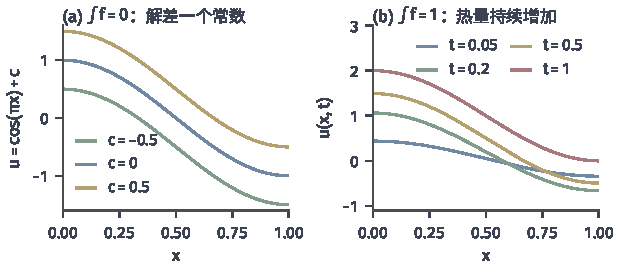
\includegraphics[width=105mm]{figures/03-optimization-evolution-and-signals/02-processes-and-trajectory-evolution/matplotlib/pde-neumann/figure.pdf}
  \caption{两端绝热的棒。(a)~$f=\pi^2\cos(\pi x)$满足相容条件$\int_0^1f=0$，$\cos(\pi x)+c$对每个常数$c$都是解。(b)~$f=1+\pi^2\cos(\pi x)$不满足相容条件；从零初温出发的热方程$u_t=u_{xx}+f$的解为$u=t+(1-e^{-\pi^2t})\cos(\pi x)$，形状趋于$\cos(\pi x)$，平均温度按$t$增长。}
  \label{fig:pde-neumann}
\end{figure}

\paragraph{零均值空间中的唯一解}
为了去掉常数方向，把解限制在均值为零的函数中，Poincaré不等式的零均值形式恰好提供所需的强制性。

\begin{theorem}[Neumann问题的弱解]
\label{thm:pde-neumann}
设$\Omega$为有界连通Lipschitz区域，$f\in L^2(\Omega)$，$g\in L^2(\partial\Omega)$。Neumann问题~\eqref{eq:pde-weak-neumann}有弱解当且仅当相容条件~\eqref{eq:pde-neumann-compatibility}成立；此时弱解在相差常数的意义下唯一，在$V=\{v\in H^1(\Omega):\int_\Omega v\,\mathrm d\bm x=0\}$中恰有一个。
\end{theorem}

\begin{proof}
必要性已由$v=1$得到。设相容条件成立。$v\mapsto\int_\Omega v$在$H^1$上连续，所以$V$是闭子空间，本身是Hilbert空间。对$v\in V$，零均值的Poincaré不等式给出$\|v\|\leq C\|\nabla v\|$，于是$\|v\|_{H^1}^2\leq(1+C^2)\|\nabla v\|^2=(1+C^2)a(v,v)$，$a$在$V$上强制。式~\eqref{eq:pde-weak-neumann}的右端$\ell$在$V$上有界，由定理~\ref{thm:pde-lax-milgram}存在唯一$u\in V$使$a(u,v)=\ell(v)$对$v\in V$成立。

还需验证对所有$v\in H^1(\Omega)$成立。把$v$写成$v=(v-v_\Omega)+v_\Omega$，第一项属于$V$；对常数$v_\Omega$，$a(u,v_\Omega)=0$，而$\ell(v_\Omega)=v_\Omega\bigl(\int_\Omega f+\int_{\partial\Omega}g\bigr)=0$正是相容条件。所以$u$是弱解。若$u_1,u_2$都是弱解，差$w$满足$a(w,w)=0$，$\nabla w=0$，在连通区域上$w$是常数。
\end{proof}

区域不连通时，每个连通分支都有自己的常数方向和自己的相容条件。定理中的连通性不能省略，与Poincaré不等式的零均值形式需要连通性是同一个原因。

\paragraph{Robin边界：边界项进入双线性型}
Robin条件$\partial_{\bm n}u+\alpha u=g$（取$\kappa=1$）把$\partial_{\bm n}u=g-\alpha u$代入Green恒等式的边界项，得到弱形式
\begin{equation}
  \begin{aligned}
    a_R(u,v)&:=\int_\Omega\nabla u\cdot\nabla v\,\mathrm d\bm x+\int_{\partial\Omega}\alpha\operatorname{Tr}u\operatorname{Tr}v\,\mathrm dS\\
    &=\int_\Omega fv\,\mathrm d\bm x+\int_{\partial\Omega}g\operatorname{Tr}v\,\mathrm dS,\qquad v\in H^1(\Omega).
  \end{aligned}
  \label{eq:pde-weak-robin}
\end{equation}
边界条件的一半进入了右端，另一半进入了双线性型。设$\alpha\in L^\infty(\partial\Omega)$，由迹定理$a_R$有界。强制性需要一个把边界值也算进来的不等式。

\begin{lemma}[带边界项的Poincaré型不等式]
\label{lem:pde-friedrichs}
设$\Omega$为有界连通Lipschitz区域。存在常数$C_F$，使所有$v\in H^1(\Omega)$满足$\|v\|^2\leq C_F\bigl(\|\nabla v\|^2+\|\operatorname{Tr}v\|_{L^2(\partial\Omega)}^2\bigr)$。
\end{lemma}

\begin{proof}
反设不成立，则有$v_n\in H^1(\Omega)$，$\|v_n\|=1$，而$\|\nabla v_n\|^2+\|\operatorname{Tr}v_n\|_{L^2(\partial\Omega)}^2<1/n$。序列在$H^1$中有界，由紧嵌入，有子列（仍记为$v_n$）在$L^2$中收敛到某个$v$，$\|v\|=1$。由于$\|v_n-v_m\|_{H^1}^2=\|v_n-v_m\|^2+\|\nabla v_n-\nabla v_m\|^2$且两项都趋于零，$(v_n)$在$H^1$中是Cauchy列，在$H^1$中收敛到$v$，$\nabla v=0$；区域连通，$v$几乎处处等于常数$c$，$|c|\,|\Omega|^{1/2}=1$。迹算子连续，$\operatorname{Tr}v_n\to\operatorname{Tr}v=c$，而$\|\operatorname{Tr}v_n\|\to0$，所以$c=0$，矛盾。
\end{proof}

若$\alpha\geq\alpha_0>0$几乎处处成立，则$a_R(v,v)\geq\min(1,\alpha_0)\bigl(\|\nabla v\|^2+\|\operatorname{Tr}v\|^2\bigr)$，由引理~\ref{lem:pde-friedrichs}，$\|v\|_{H^1}^2\leq(C_F+1)\bigl(\|\nabla v\|^2+\|\operatorname{Tr}v\|^2\bigr)$，所以$a_R$在整个$H^1(\Omega)$上强制。由定理~\ref{thm:pde-lax-milgram}，弱解存在唯一，不需要相容条件，也没有常数方向。物理上，边界只要有一点“漏热”，稳态就被唯一确定。

\paragraph{系数符号}
上面用到$\alpha\geq\alpha_0>0$。符号反过来，结论可以失效。在$(0,1)$上两端都取Robin条件，外法向在左端指向$-x$、在右端指向$+x$，条件为$-u'(0)+\alpha u(0)=0$与$u'(1)+\alpha u(1)=0$。对$-u''=0$，解为$u=A+Bx$，代入得$B=\alpha A$与$\alpha A(2+\alpha)=0$。$\alpha=-2$时$A$任意，$u=1-2x$是非零解，所以齐次问题有非零解，唯一性失败。这时$a_R(1,1)=\alpha\cdot(1+1)=-4<0$，强制性不成立。物理上$\alpha<0$意味着边界越热、从外界吸收的热量越多，这已不是Newton冷却。

\paragraph{三种边界条件的对照}
表~\ref{tab:pde-boundary-comparison}汇总了本小节的比较。同一个方程$-\Delta u=f$，边界条件一变，解空间、边界条件进入弱形式的位置、存在所需的条件以及唯一性都随之改变，不能把Dirichlet版本的结论直接搬过去。

\begin{table*}[!htb]
  \centering
  \begin{tabularx}{\linewidth}{@{}l>{\RaggedRight\arraybackslash}X>{\RaggedRight\arraybackslash}X>{\RaggedRight\arraybackslash}X@{}}
    \toprule
    边界条件 & 解空间 & 条件进入弱形式的位置 & 存在与唯一 \\
    \midrule
    Dirichlet $u=g$ & $G+H_0^1(\Omega)$ & 解空间（本质条件） & 总存在且唯一 \\
    Neumann $\partial_{\bm n}u=g$ & $H^1(\Omega)$ & 右端边界积分（自然条件） & 需相容条件，差常数 \\
    Robin $\partial_{\bm n}u+\alpha u=g$ & $H^1(\Omega)$ & 双线性型与右端 & 总存在且唯一 \\
    \bottomrule
  \end{tabularx}
  \caption{Poisson方程三种边界条件的弱形式对照（$\Omega$为有界连通Lipschitz区域，Robin情形设$\alpha\geq\alpha_0>0$）。}
  \label{tab:pde-boundary-comparison}
\end{table*}
